% ---------------------------------------------------------------------------------------------------------------------
% document class
% ---------------------------------------------------------------------------------------------------------------------
\documentclass[
    11pt,        % normal font size
    a4paper,     % paper size
    final,       % final or draft version
    fleqn,       % left-aligned equations
    notitlepage, % no seperate title and abstract pages
    onecolumn,   % single-column text
    oneside,     % single-sided output
]{article}

% ---------------------------------------------------------------------------------------------------------------------
% page geometry setup
% ---------------------------------------------------------------------------------------------------------------------
\usepackage[
    a4paper,      % paper size (A4: 21.0cm x 29.7cm)
    left=2.5cm,   % margin: left
    right=2.5cm,  % margin: right
    top=3.5cm,    % margin: top
    bottom=3.5cm, % margin: bottom
]{geometry}

% ---------------------------------------------------------------------------------------------------------------------
% font options
% ---------------------------------------------------------------------------------------------------------------------
\usepackage{fontspec}       % for OpenType fonts (requires compilation with LuaTeX)
\usepackage{unicode-math}   % for unicode maths  (requires compilation with LuaTeX)
\setmainfont{STIX Two Text} % main font
\setmathfont{STIX Two Math} % math font

% ---------------------------------------------------------------------------------------------------------------------
% hyperlinks
% ---------------------------------------------------------------------------------------------------------------------
\usepackage[
    colorlinks=true,   % use coloured links
    allcolors=magenta, % use a single link colour
]{hyperref}

% ---------------------------------------------------------------------------------------------------------------------
% images and graphics
% ---------------------------------------------------------------------------------------------------------------------
\usepackage{graphicx,tikz}
\usetikzlibrary{arrows.meta}

% ---------------------------------------------------------------------------------------------------------------------
% begin document
% ---------------------------------------------------------------------------------------------------------------------
\begin{document}

% ---------------------------------------------------------------------------------------------------------------------
% title
% ---------------------------------------------------------------------------------------------------------------------
\begin{center}
    \bfseries
    \huge
    FeaSoft quick start guide
\end{center}

\begin{center}
    \bfseries
    \large
    Version 1.0
\end{center}

\begin{center}
    \bfseries
    \large
    \url{https://github.com/FeaSoft/App}
\end{center}

\begin{center}
    \large
    Carlos Souto\footnote{Email address: \href{mailto:csouto@fe.up.pt}{csouto@fe.up.pt} (C. Souto).}

    \vspace{5pt}
    \normalsize
    Faculty of Engineering \\ University of Porto
\end{center}

\begin{center}
    \large
    \today
\end{center}

% ---------------------------------------------------------------------------------------------------------------------
% table of contents
% ---------------------------------------------------------------------------------------------------------------------
\tableofcontents

% ---------------------------------------------------------------------------------------------------------------------
% introduction
% ---------------------------------------------------------------------------------------------------------------------
\section{Introduction}

This document is a quick start guide for the FeaSoft software application aiming to introduce the user to the software's basic functionality. To this end, this guide presents tutorials on how to use the software. However, before the tutorials, a quick description of what FeaSoft is and is not is shown below.

\subsection{What is FeaSoft}

FeaSoft is an open-source software application for performing linear perturbation analyses on solids via the finite element method with built-in capabilities for visualizing and interacting with finite element models and results. These linear perturbation analyses consist of static, frequency, and buckle analyses. Several finite elements are implemented, which can be applied in plane stress, plane strain, axisymmetric, and general three-dimensional cases. Distinct loading conditions can be modelled via the application of concentrated nodal loads, distributed surface loads (namely, pressures and surface tractions), and inertia loads (namely, body forces and accelerations, e.g., due to gravity).

As originally distributed, FeaSoft consists of three main programs:
\begin{itemize}
    \item fs\textunderscore app.exe is the main application including the graphical user interface. The user interface is built using Python, mainly relying on the PySide6 package, which provides access to the Qt framework used for the application development, and on the VTK package, which provides access to the Visualization Toolkit used for rendering. The fs\textunderscore app.exe file itself is built using the PyInstaller package. These packages are open-source and freely available.
    \item fs\textunderscore solver.exe is the main solver program. It is written in Fortran and built using the Intel Fortran Compiler, which enables automatic optimizations based on vectorization and parallel execution. Additionally, the solver relies on the Intel Math Kernel Library for fast computational routines. All Intel oneAPI Toolkits products are freely available and open-source. Moreover, the sparsity of the algebraic systems arising from finite element analyses is accounted for via a custom implementation of storage for sparse matrices.
    \item fs\textunderscore preprocessor.exe connects fs\textunderscore app.exe to fs\textunderscore solver.exe. It performs checks on the user-built models to ensure some basic integrity and minimize runtime errors during the solver execution. After checking the model created using the main application, the preprocessor also converts the data into a job file which is then treated as an input for the solver. The preprocessor is written in Python and is built using the aforementioned PyInstaller package.
\end{itemize}

\subsection{What FeaSoft is not}

FeaSoft is not a mesh generator nor a CAD software and the user may not use it to define physical geometries nor to generate meshes. Instead, the physical geometry to be analysed must first be discretized into a finite element mesh. Ultimately, this means that FeaSoft requires a mesh input file in order to create a new finite element model.

\subsection{How to generate a mesh input file}

Currently, FeaSoft expects an Abaqus input file (*.inp) as a mesh input file. There are several ways to generate this file:
\begin{enumerate}
    \item For sufficiently simple meshes, one may write this file directly using a text editor or generate it via a scripting language (e.g., Python or Matlab).
    \item For larger and more complex meshes, one may use Abaqus to define the physical geometry and then generate the mesh. This is not a particularly interesting way since Abaqus is paid software and the user may run a finite element analysis directly in this software, nullifying the need for FeaSoft.
    \item The recommended way is to generate the finite element mesh via Gmsh (or other mesh generator). Gmsh is freely available and open-source. Gmsh has a built-in CAD engine, so it can be used to define the physical geometry and then a mesh can be generated. However, Gmsh can also be used as a meshing tool only, leaving the task of defining the physical geometry to another CAD software (e.g., FreeCAD). Gmsh is capable of exporting the generated mesh as an Abaqus input file.
\end{enumerate}

Alternatively, for sufficiently simple meshes, one may skip generating a mesh input file and create a FeaSoft finite element model database directly. FeaSoft model database files (*.fs\textunderscore mdb) are pure Python files that are interpreted at runtime and can be created using a text editor. FeaSoft output database files (*.fs\textunderscore odb) are also pure Python files. As an example on how model and output databases are defined, see the example files provided in the original distribution of FeaSoft.

% ---------------------------------------------------------------------------------------------------------------------
% tutorials
% ---------------------------------------------------------------------------------------------------------------------

\section{Usage examples}

The following consists of a series of examples on how to use FeaSoft to perform finite element analyses. As previously discussed, FeaSoft requires a mesh input file of the discretized physical geometry that is to be analysed. Based on this file, a FeaSoft model database will automatically be created and opened in the main application. The user may then define node sets, element sets, and surface sets by interacting with the model\footnote{Although node sets and element sets can be defined in FeaSoft, it is often more convenient to define these during the meshing process, e.g., via Gmsh's physical groups.}. Node sets are used to apply concentrated nodal loads and boundary conditions in the form of prescribed nodal displacements. Element sets are used to define sections, which in turn assign materials and stress states to the finite elements; element sets are also used to apply inertia loads in the form of body forces and accelerations. Finally, surface sets are used for the definition of distributed surface loads, namely, pressures and surface tractions.

Once a finite element model has been defined by the user, a job may be submitted to the solver, which will generate an output database. The results may then be opened in the main application.

\subsection{Static analysis of a plate with a central hole}

Consider the following problem:
\begin{center}
    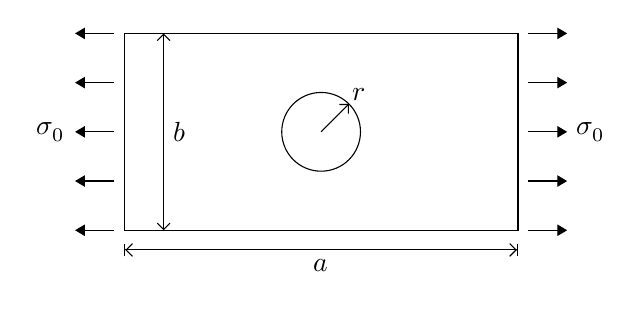
\begin{tikzpicture}[scale=0.25]
        \draw (0,0) rectangle (20,10);
        \draw (10,5) circle (2);
        \draw[-Triangle] (-0.5,0.0) -- ++(180:2);
        \draw[-Triangle] (-0.5,2.5) -- ++(180:2);
        \draw[-Triangle] (-0.5,5.0) -- ++(180:2) node[left]{$\sigma_0$};
        \draw[-Triangle] (-0.5,7.5) -- ++(180:2);
        \draw[-Triangle] (-0.5,10.) -- ++(180:2);
        \draw[-Triangle] (20.5,0.0) -- ++(0:2);
        \draw[-Triangle] (20.5,2.5) -- ++(0:2);
        \draw[-Triangle] (20.5,5.0) -- ++(0:2) node[right]{$\sigma_0$};
        \draw[-Triangle] (20.5,7.5) -- ++(0:2);
        \draw[-Triangle] (20.5,10.) -- ++(0:2);
        \draw[{Bar}{Straight Barb}-{Straight Barb}{Bar}] (0,-1) -- (20,-1) node[midway,below]{$a$};
        \draw[{Straight Barb}-{Straight Barb}] (2,0) -- (2,10) node[midway,right]{$b$};
        \draw[-{Straight Barb}] (10,5) -- ++(45:2) node[above right,inner sep=1]{$r$};
    \end{tikzpicture}
\end{center}
The geometry of the plate is defined by a length of $a = 200$ mm, a width of $b = 100$ mm, and a thickness of $t = 10$ mm. The central hole is defined by a radius of $r = 20$ mm. The material is considered linear-elastic, defined by a Young's modulus of $E = 210$ GPa and a Poisson's ratio of $\nu = 0.3$. The applied tension has a magnitude of $\sigma_0 = 250$ MPa. A plane stress condition is assumed.

\textbf{Important:} before starting the model definition, always remember that FeaSoft, like other finite element applications (e.g., Abaqus), assumes that consistent units are used. For this example, the geometric properties are specified in mm, while the Young's modulus and applied tension are specified in MPa, i.e., N/mm\textsuperscript{2}. Consequently, displacements will be computed in mm, forces will be computed in N, and stresses will be computed in MPa.

To start the model definition in FeaSoft, go to File > New...\ and open the pre-prepared mesh input file named plate-hole.inp found in the examples/1 directory. The application should warn that a model database already exists in the directory; press Yes on the dialog box to proceed. The newly created model database should be displayed in the interface as shown:
\begin{center}
    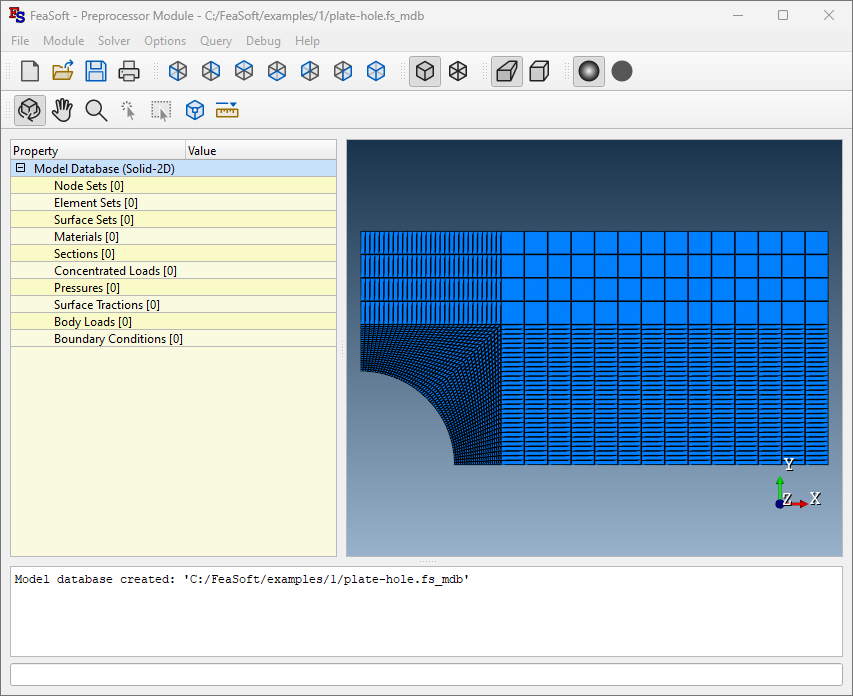
\includegraphics[scale=0.5]{fig/ui-1-1.png}
\end{center}

In the model tree, right-click on the Node Sets tree item and click the Add item on the context menu to create a new node set:
\begin{center}
    \begin{tikzpicture}
        \node[inner sep=0] at (0,0) {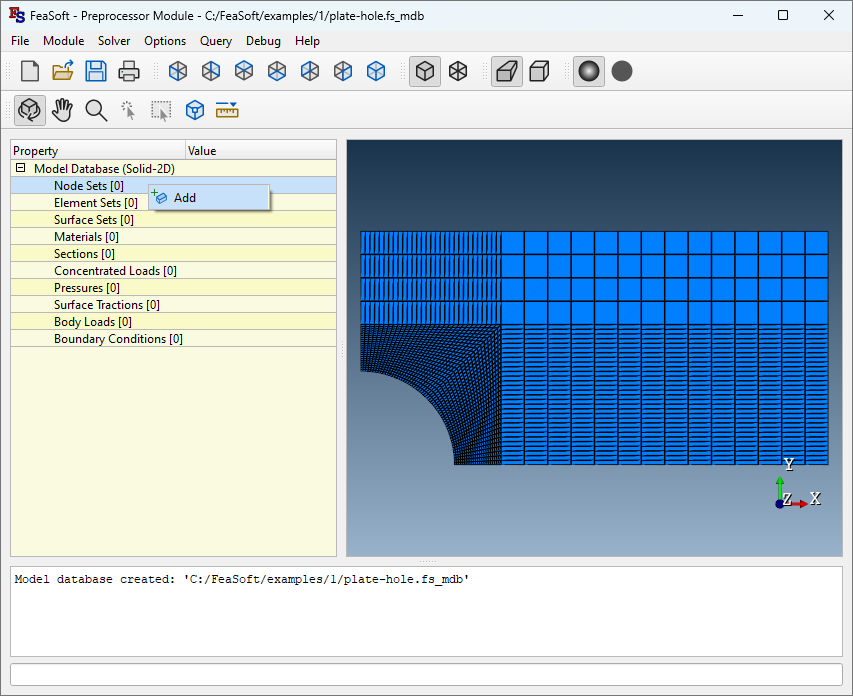
\includegraphics[scale=0.5]{fig/ui-1-2.png}};
        \draw[red] (-5.55,1.7) rectangle (-1.15,2.8);
    \end{tikzpicture}
\end{center}

Expand the Node Sets and Node-Set-1 tree items. Edit the Name property of the node set Node-Set-1; input X-BC as the new name of the node set and press Enter to finalize the edit:
\begin{center}
    \begin{tikzpicture}
        \node[draw=red,inner sep=0.5] at (0,0) {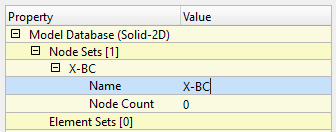
\includegraphics[scale=1]{fig/ui-1-3.png}};
    \end{tikzpicture}
\end{center}

While the node set X-BC tree item is selected (or any of its child items), the viewport pickers toolbar buttons will be enabled; select the Pick Multiple toolbar button:
\begin{center}
    \begin{tikzpicture}
        \node[inner sep=0] at (0,0) {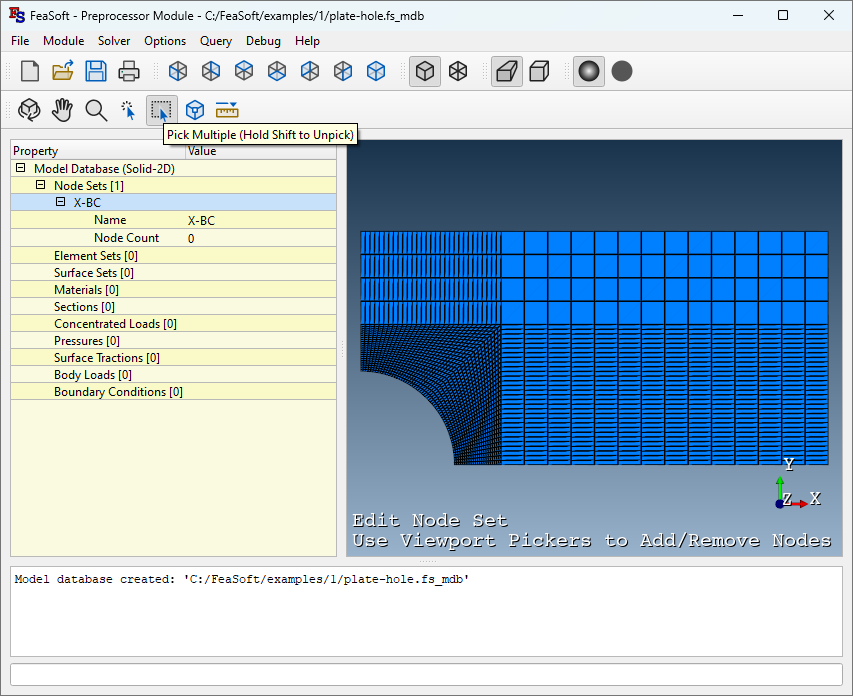
\includegraphics[scale=0.5]{fig/ui-1-4.png}};
        \draw[red] (-5.55,1.35) rectangle (-0.85,3.4);
    \end{tikzpicture}
\end{center}

Select the following edge nodes; exactly 27 nodes should be selected (shown by the Node Count property in the model tree):
\begin{center}
    \begin{tikzpicture}
        \node[inner sep=0] at (0,0) {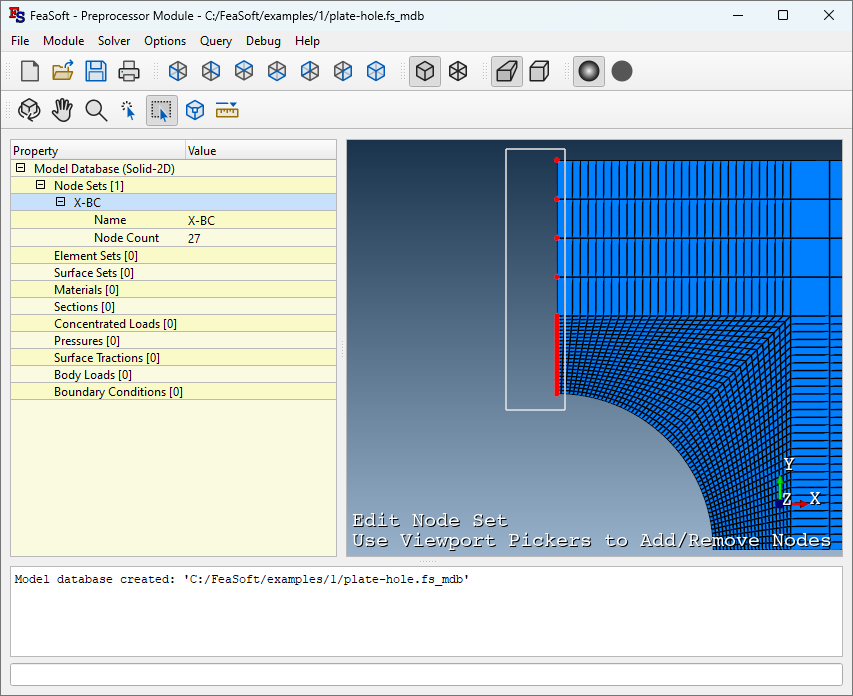
\includegraphics[scale=0.5]{fig/ui-1-5.png}};
        \draw[red] (-5.55,1.34) rectangle (-1.15,2.05);
    \end{tikzpicture}
\end{center}

Repeating the same process used to create the X-BC node set, create the Y-BC node set with the following 37 edge nodes:
\begin{center}
    \begin{tikzpicture}
        \node[inner sep=0] at (0,0) {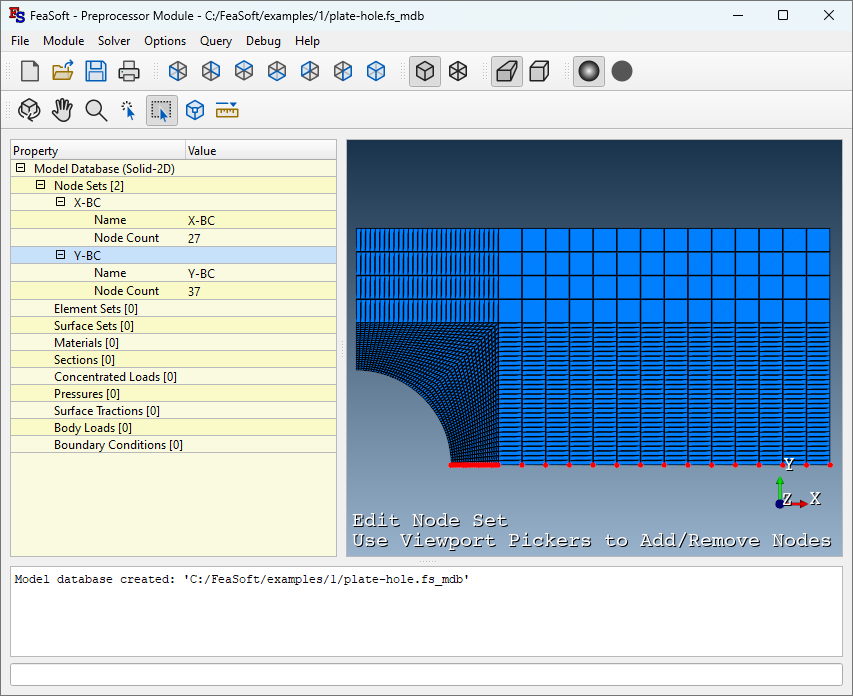
\includegraphics[scale=0.5]{fig/ui-1-6.png}};
        \draw[red] (-5.55,0.64) rectangle (-1.15,2.05);
    \end{tikzpicture}
\end{center}

In the model tree, right-click on the Element Sets tree item and click the Add item on the context menu to create a new element set:
\begin{center}
    \begin{tikzpicture}
        \node[inner sep=0] at (0,0) {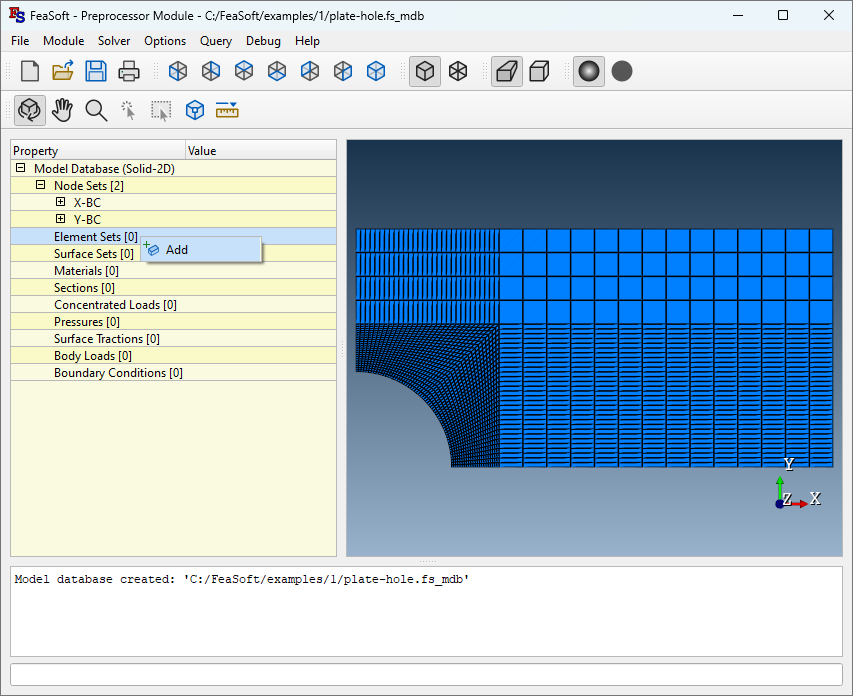
\includegraphics[scale=0.5]{fig/ui-1-7.png}};
        \draw[red] (-5.55,1.1) rectangle (-1.15,1.65);
    \end{tikzpicture}
\end{center}

Rename the newly created Elment-Set-1 to All-Elements and select all elements using the Pick Multiple viewport picker; exactly 1916 elements should be selected (shown by the Element Count property in the model tree):
\begin{center}
    \begin{tikzpicture}
        \node[inner sep=0] at (0,0) {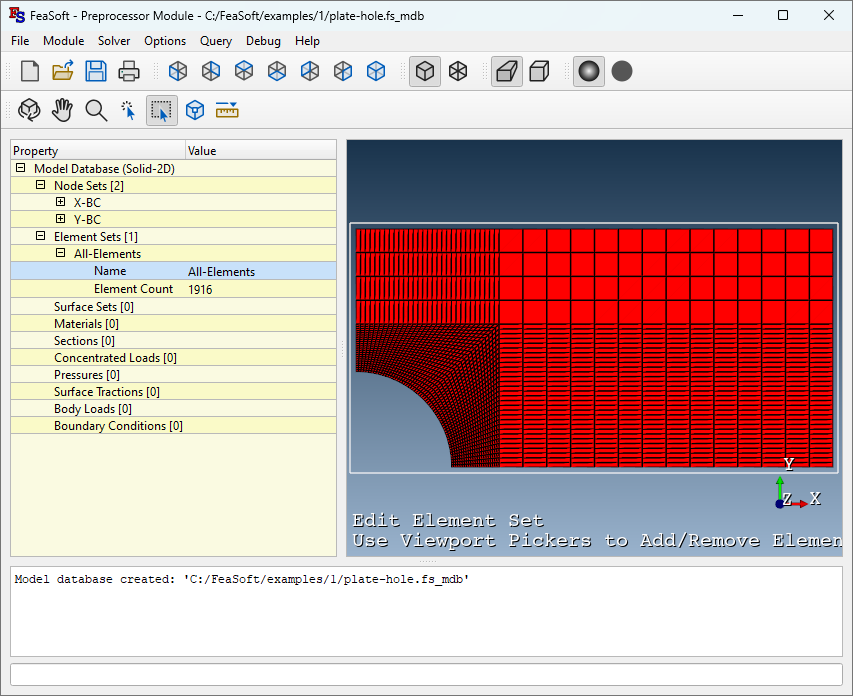
\includegraphics[scale=0.5]{fig/ui-1-8.png}};
        \draw[red] (-5.55,0.6) rectangle (-1.15,1.65);
        \draw[red] (-4.2,2.9) rectangle (-3.2,3.4);
    \end{tikzpicture}
\end{center}

Following the same procedure used to create node sets and element sets, create the following surface set named Load-Surface\footnote{Surfaces are selected by picking the nodes that define them using the Pick Multiple viewport picker.}, which contains exactly 34 surfaces (shown by the Surface Count property in the model tree):
\begin{center}
    \begin{tikzpicture}
        \node[inner sep=0] at (0,0) {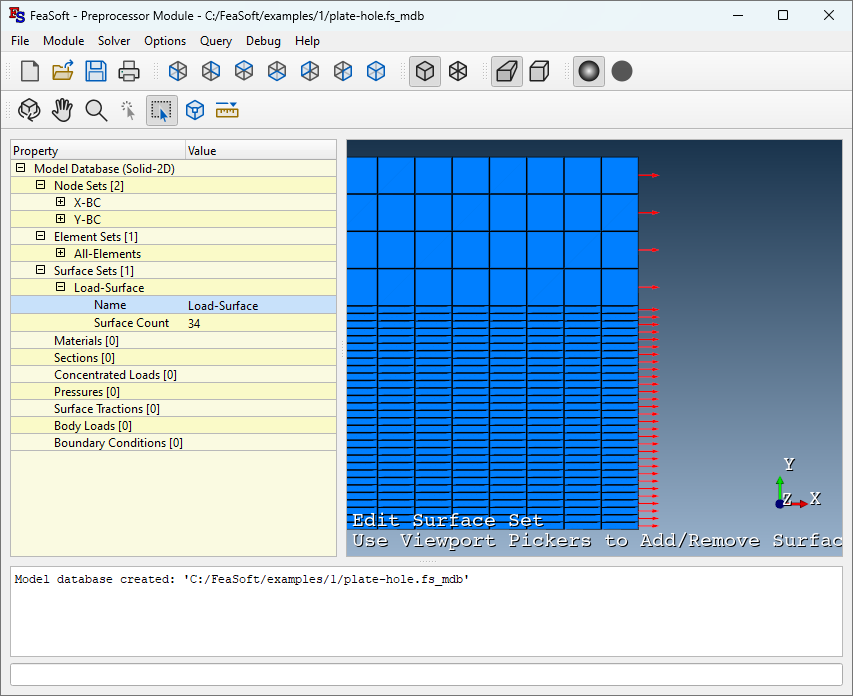
\includegraphics[scale=0.5]{fig/ui-1-9.png}};
        \draw[red] (-5.55,0.2) rectangle (-1.15,1.15);
        \draw[red] (-3.8,2.9) rectangle (-3.2,3.4);
    \end{tikzpicture}
\end{center}

In the model tree, right-click on the Materials tree item and click the Add item on the context menu to create a new material. Rename the material to Steel and define its properties as shown\footnote{A static analysis without inertia loads in the form of accelerations (e.g., due to gravity) does not require the material's mass density property to be defined.}:
\begin{center}
    \begin{tikzpicture}
        \node[draw=red,inner sep=0.5] at (0,0) {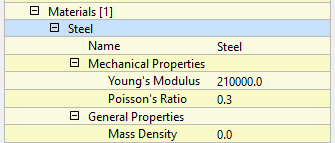
\includegraphics[scale=1]{fig/ui-1-10.png}};
    \end{tikzpicture}
\end{center}

In the model tree, right-click on the Sections tree item and click the Add item on the context menu to create a new section. Rename the section to Solid-Section; assign the Steel material, the 2D Plane Stress stress state, and a Plane Thickness to the All-Elements element set:
\begin{center}
    \begin{tikzpicture}
        \node[draw=red,inner sep=0.5] at (0,0) {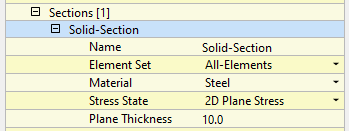
\includegraphics[scale=1]{fig/ui-1-11.png}};
    \end{tikzpicture}
\end{center}

In the model tree, right-click on the Surface Tractions tree item and click the Add item on the context menu to create a new surface traction. Rename the surface traction to Tension-Load and assign it to the Load-Surface surface set; define the load components as follows:
\begin{center}
    \begin{tikzpicture}
        \node[draw=red,inner sep=0.5] at (0,0) {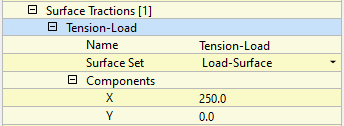
\includegraphics[scale=1]{fig/ui-1-12.png}};
    \end{tikzpicture}
\end{center}
\begin{center}
    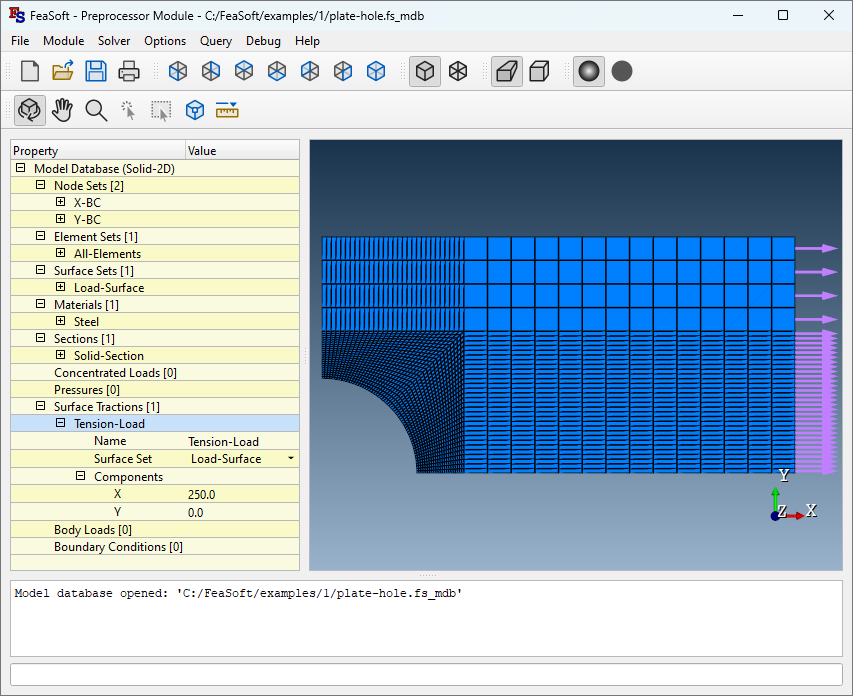
\includegraphics[scale=0.5]{fig/ui-1-13.png}
\end{center}

In the model tree, right-click on the Boundary Conditions tree item and click the Add item on the context menu to create a new boundary condition. Rename the boundary condition to X-Symmetry and assign it to the X-BC node set; activate the X degree of freedom as shown:
\begin{center}
    \begin{tikzpicture}
        \node[draw=red,inner sep=0.5] at (0,0) {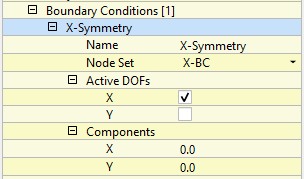
\includegraphics[scale=1]{fig/ui-1-14.png}};
    \end{tikzpicture}
\end{center}
\begin{center}
    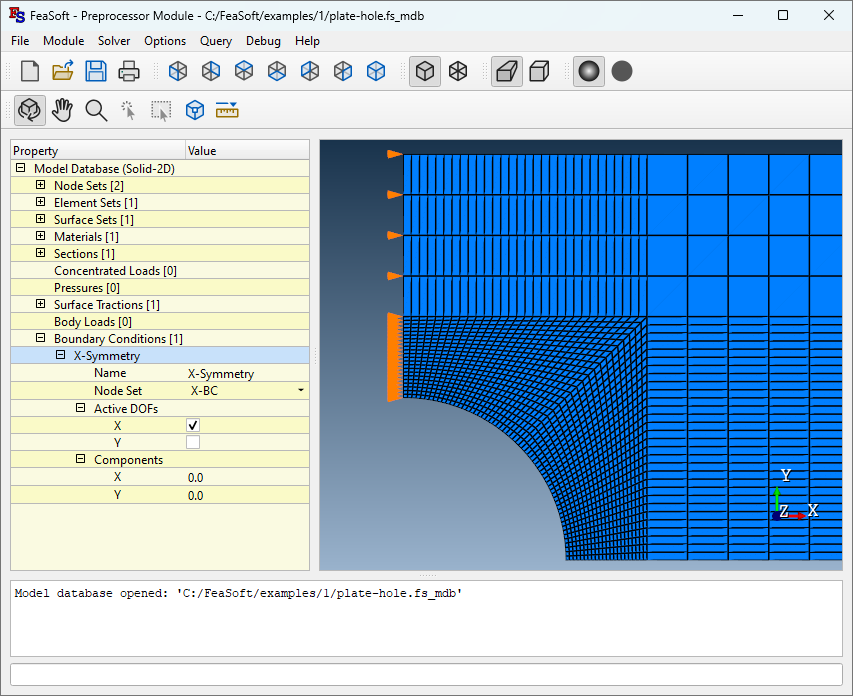
\includegraphics[scale=0.5]{fig/ui-1-15.png}
\end{center}

In the model tree, right-click on the Boundary Conditions tree item and click the Add item on the context menu to create a new boundary condition. Rename the boundary condition to Y-Symmetry and assign it to the Y-BC node set; activate the Y degree of freedom as shown:
\begin{center}
    \begin{tikzpicture}
        \node[draw=red,inner sep=0.5] at (0,0) {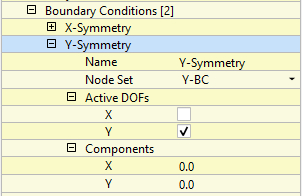
\includegraphics[scale=1]{fig/ui-1-16.png}};
    \end{tikzpicture}
\end{center}
\begin{center}
    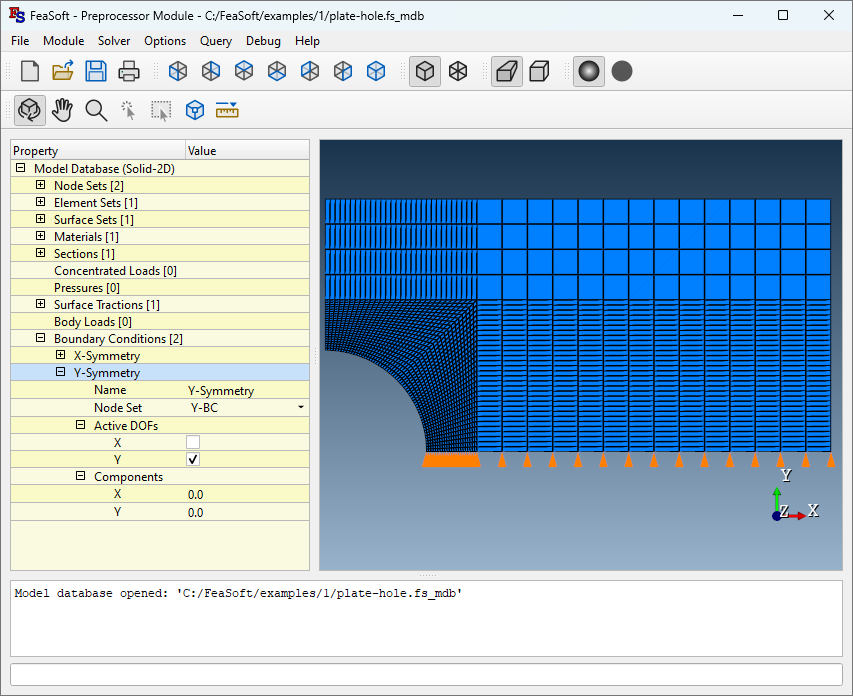
\includegraphics[scale=0.5]{fig/ui-1-17.png}
\end{center}

\textbf{Important:} since the model has been completely defined, it is necessary to save it now (File > Save or via the Save Model Database toolbar button) before submitting the job to the solver; the preprocessor will always consider the last saved state of the model (unsaved changes are ignored for the analysis).

Once the model has been saved, go to Solver > Submit and select the plate-hole.fs\textunderscore mdb model database file:
\begin{center}
    \begin{tikzpicture}
        \node[inner sep=0] at (0,0) {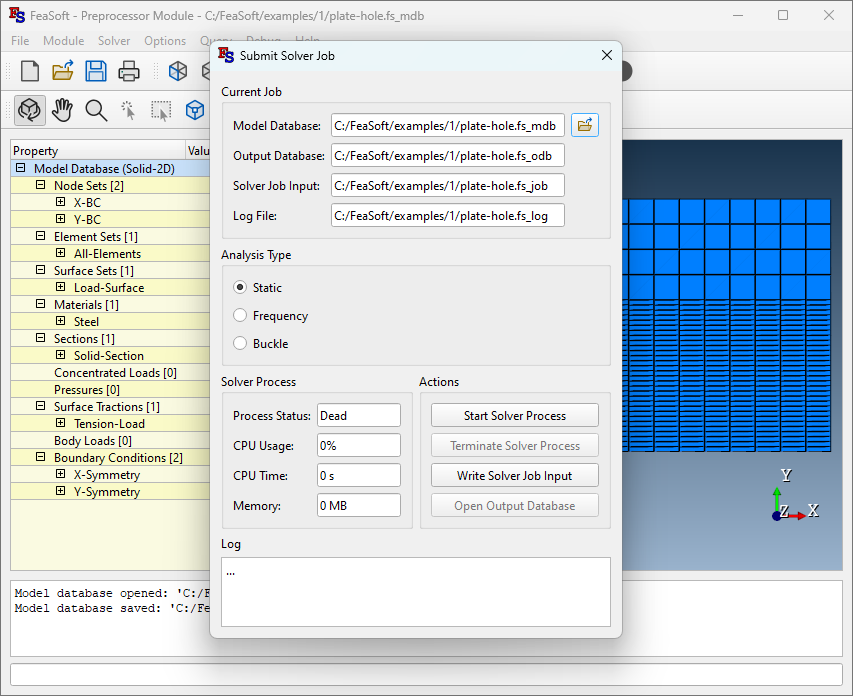
\includegraphics[scale=0.5]{fig/ui-1-18.png}};
        \draw[red] (-2.75,1.4) rectangle (2.5,3.55);
    \end{tikzpicture}
\end{center}

Once a model database has been specified for the analysis, the procedure can be started by clicking on the Start Solver Process button. While the preprocessor and solver are running, the Process Status box will show the Alive process flag; the Dead process flag will be shown while the preprocessor and solver are not running. The analysis is successfully completed once the ``Solver is done'' message is shown on the bottom of the Log:
\begin{center}
    \begin{tikzpicture}
        \node[draw=red,inner sep=0.5] at (0,0) {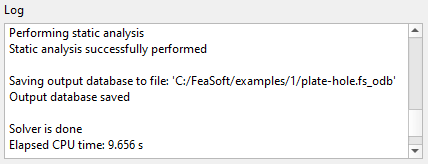
\includegraphics[scale=1]{fig/ui-1-19.png}};
    \end{tikzpicture}
\end{center}

At this point, the output database can be opened by clicking on the Open Output Database button (or via the File > Open...\ menu action). On the output tree, expand the Field Output, Frame 1, and Stress tree items. Click on the Mises Equivalent Stress tree item to plot this nodal scalar field:
\begin{center}
    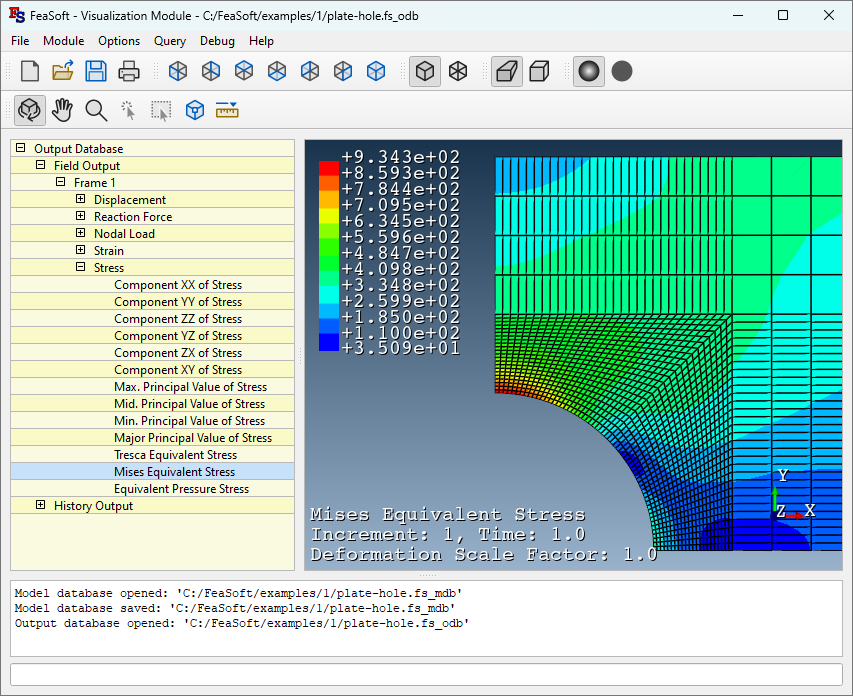
\includegraphics[scale=0.5]{fig/ui-1-20.png}
\end{center}

Several options can be adjusted on the Options > Common and Options > Result dialogs. The viewport can also be printed via the File > Print...\ menu action or the Print Viewport toolbar button. An example on how the results can be presented is shown below:
\begin{center}
    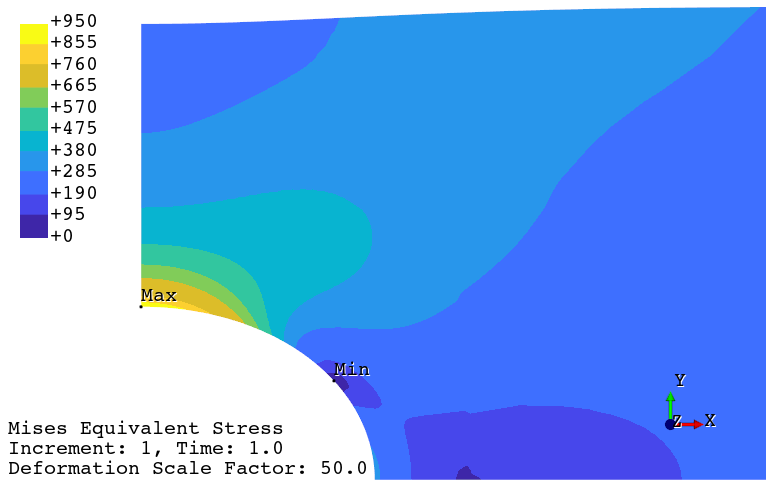
\includegraphics[scale=0.5]{fig/ui-1-21.png}
\end{center}

\subsection{Static analysis of a pressure vessel}

The following illustration represents the cross-section of an axisymmetric pressure vessel:
\begin{center}
    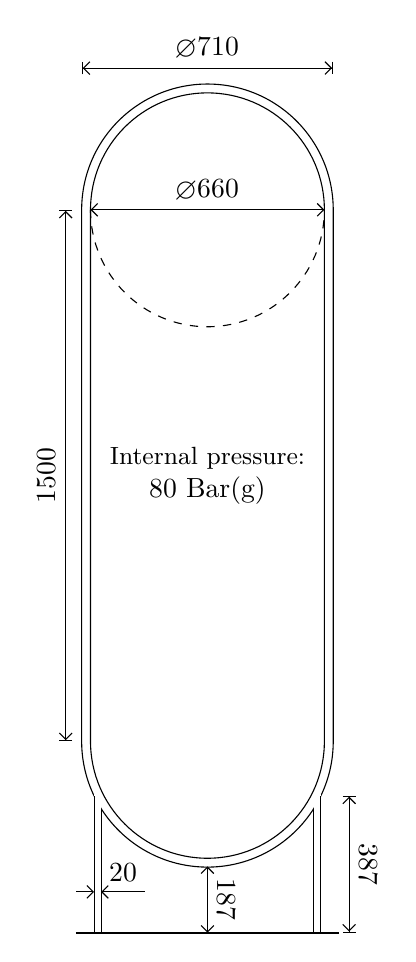
\begin{tikzpicture}[scale=4.5]
        \draw (-0.355,0) arc (180:360:0.355) -- ++(0,1.5) arc (0:180:0.355) -- cycle;
        \fill[white] (+0.3,-0.09) -- ++(0,-0.45) -- ++(+0.02,0) -- ++(0,0.45) -- cycle;
        \fill[white] (-0.3,-0.09) -- ++(0,-0.45) -- ++(-0.02,0) -- ++(0,0.45) -- cycle;
        \draw (-0.33,0) arc (180:360:0.33) -- ++(0,1.5) arc (0:180:0.33) -- cycle;
        \draw[dashed] (-0.33,1.5) arc (180:360:0.33);
        \draw (+0.3,-0.19) -- ++(0,-0.35) -- ++(+0.02,0) -- ++(0,0.387);
        \draw (-0.3,-0.19) -- ++(0,-0.35) -- ++(-0.02,0) -- ++(0,0.387);
        \draw[thick] (-0.371,-0.54) -- (+0.371,-0.54);
        \node[align=center] at (0,0.75) {\small Internal pressure:\\$80$ Bar(g)};
        \draw[{Bar}{Straight Barb}-{Straight Barb}{Bar}] (+0.4,-0.54) -- ++(0,0.387) node[midway,rotate=-90,above]{$387$};
        \draw[{Bar}{Straight Barb}-{Straight Barb}{Bar}] (-0.4,0) -- ++(0,1.5) node[midway,rotate=90,above]{$1500$};
        \draw[{Bar}{Straight Barb}-{Straight Barb}{Bar}] (-0.355,1.9) -- ++(0.71,0) node[midway,above]{$\diameter 710$};
        \draw[{Straight Barb}-{Straight Barb}] (-0.33,1.5) -- ++(0.66,0) node[midway,above]{$\diameter 660$};
        \draw[{Straight Barb}-{Straight Barb}] (0,-0.54) -- ++(0,0.187) node[midway,rotate=-90,above]{$187$};
        \draw[{Straight Barb}-] (-0.32,-0.425) -- ++(180:0.05);
        \draw[{Straight Barb}-] (-0.3,-0.425) -- ++(0:0.125) node[midway,above]{$20$};
    \end{tikzpicture}
\end{center}
The geometrical dimensions are shown in mm. The material is considered linear-elastic, defined by a Young's modulus of $E = 210$ GPa, a Poisson's ratio of $\nu = 0.3$, and a density of $\rho = 7.85$ g/cm\textsuperscript{3}. The internal pressure has a magnitude of 80 Bar(g). An axisymmetric stress state is assumed. The self-weight of the vessel should be considered in the analysis.

\textbf{Important:} before starting the model definition, always remember that FeaSoft, like other finite element applications (e.g., Abaqus), assumes that consistent units are used. For this example, the geometric properties are specified in mm, while the Young's modulus and internal pressure are specified in MPa, i.e., N/mm\textsuperscript{2}; moreover, the acceleration due to gravity is specified in mm/s\textsuperscript{2} and the density is specified in t/mm\textsuperscript{3}. Consequently, displacements will be computed in mm, forces will be computed in N, and stresses will be computed in MPa.

To start the model definition in FeaSoft, go to File > New...\ and open the pre-prepared mesh input file named pressure-vessel.inp found in the examples/2 directory. The application should warn that a model database already exists in the directory; press Yes on the dialog box to proceed. The newly created model database should be displayed in the interface as shown:
\begin{center}
    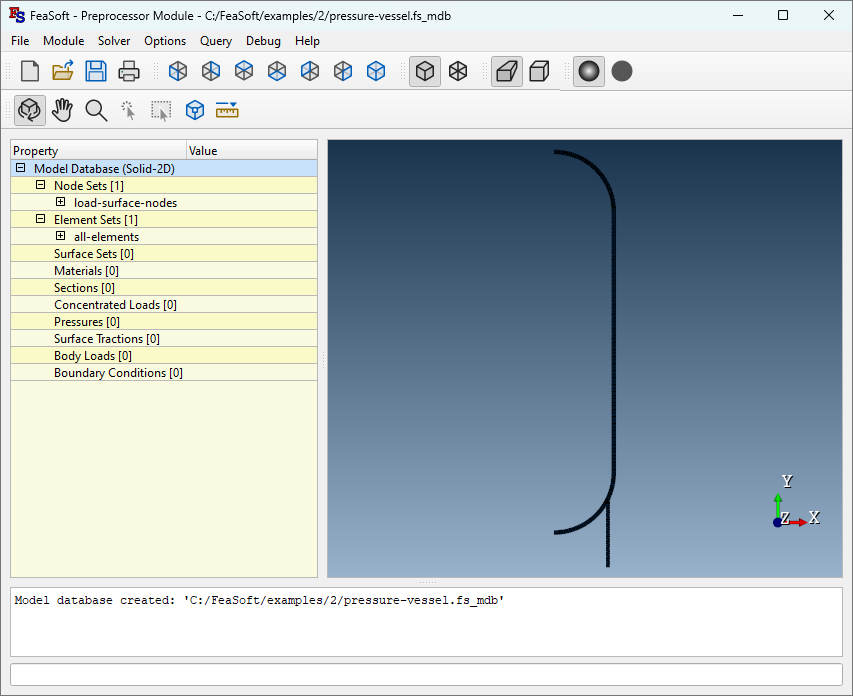
\includegraphics[scale=0.5]{fig/ui-2-1.png}
\end{center}
Notice that a node set and an element set are already present in the model database as they were defined during the meshing process.

To apply the internal pressure (a distributed surface load), a surface set is first required. To create the surface set, right-click on the load-surface-nodes node set tree item and click on the Convert to Surface Set context menu item:
\begin{center}
    \begin{tikzpicture}
        \node[draw=red,inner sep=0.5] at (0,0) {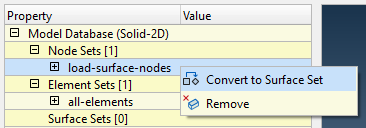
\includegraphics[scale=1]{fig/ui-2-2.png}};
    \end{tikzpicture}
\end{center}

Rename the new surface set to load-surface:
\begin{center}
    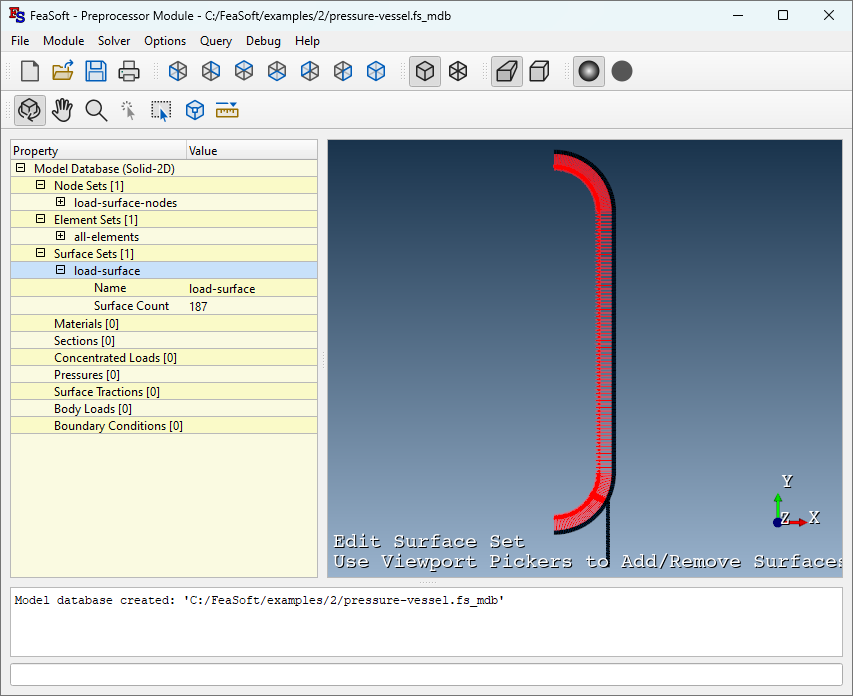
\includegraphics[scale=0.5]{fig/ui-2-3.png}
\end{center}

Following the same procedure used in the first example, create the following material:
\begin{center}
    \begin{tikzpicture}
        \node[draw=red,inner sep=0.5] at (0,0) {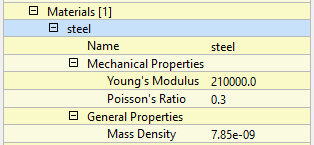
\includegraphics[scale=1]{fig/ui-2-4.png}};
    \end{tikzpicture}
\end{center}

Following the same procedure used in the first example, create the following section\footnote{The Plane Thickness property is ignored for a 2D Axisymmetric stress state.}:
\begin{center}
    \begin{tikzpicture}
        \node[draw=red,inner sep=0.5] at (0,0) {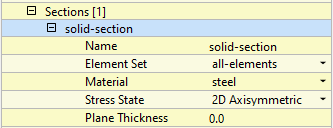
\includegraphics[scale=1]{fig/ui-2-5.png}};
    \end{tikzpicture}
\end{center}

Create the following pressure:
\begin{center}
    \begin{tikzpicture}
        \node[draw=red,inner sep=0.5] at (0,0) {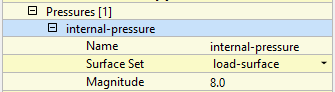
\includegraphics[scale=1]{fig/ui-2-6.png}};
    \end{tikzpicture}
\end{center}
\begin{center}
    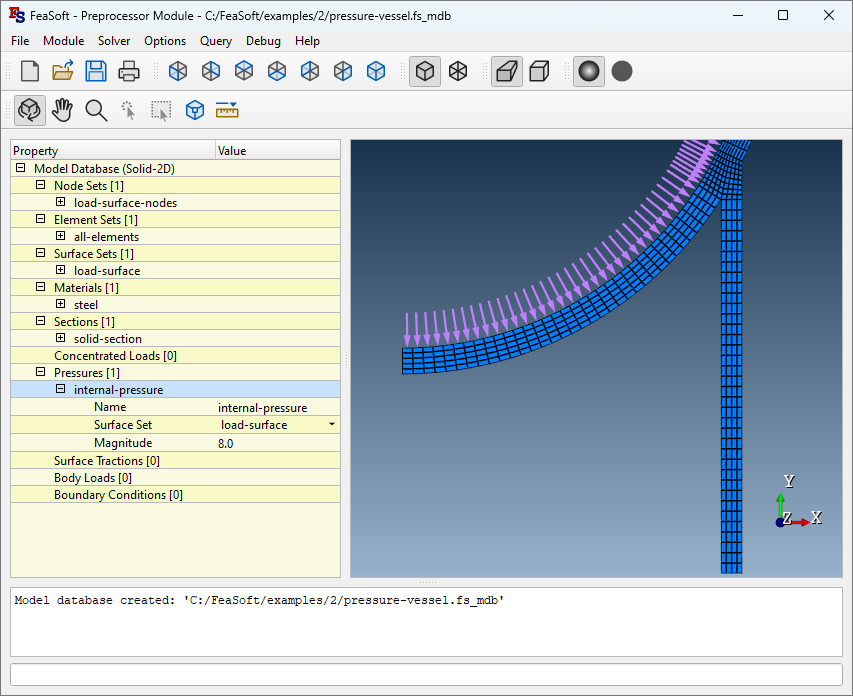
\includegraphics[scale=0.5]{fig/ui-2-7.png}
\end{center}

Create the following body load:
\begin{center}
    \begin{tikzpicture}
        \node[draw=red,inner sep=0.5] at (0,0) {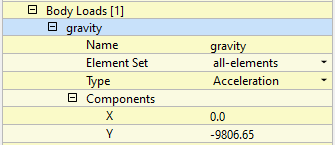
\includegraphics[scale=1]{fig/ui-2-8.png}};
    \end{tikzpicture}
\end{center}
\begin{center}
    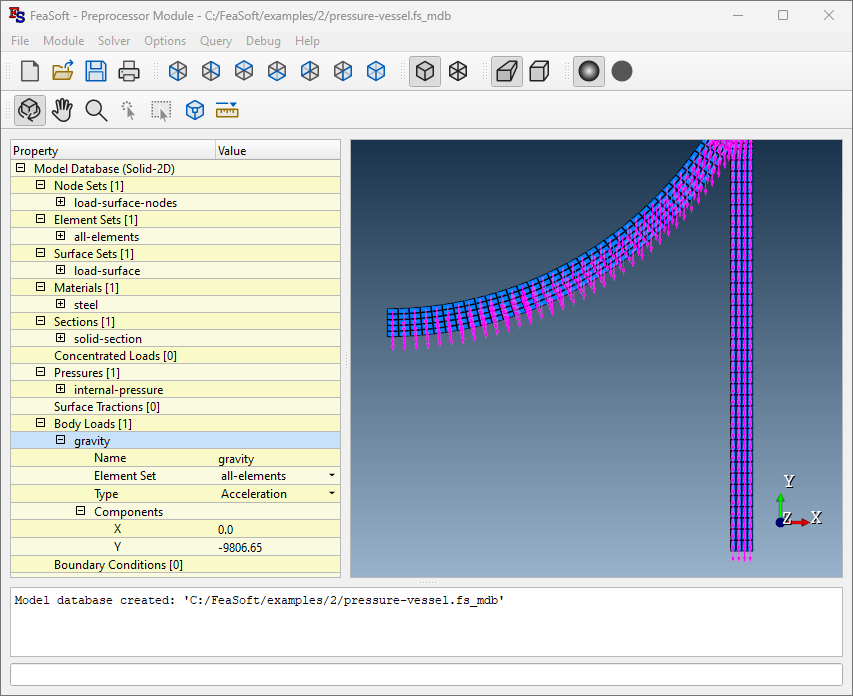
\includegraphics[scale=0.5]{fig/ui-2-9.png}
\end{center}

Lastly, create the following boundary condition:
\begin{center}
    \begin{tikzpicture}
        \node[draw=red,inner sep=0.5] at (0,0) {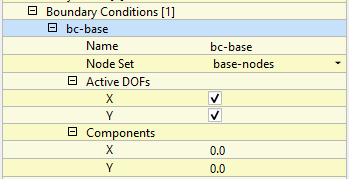
\includegraphics[scale=1]{fig/ui-2-10.png}};
    \end{tikzpicture}
\end{center}
\begin{center}
    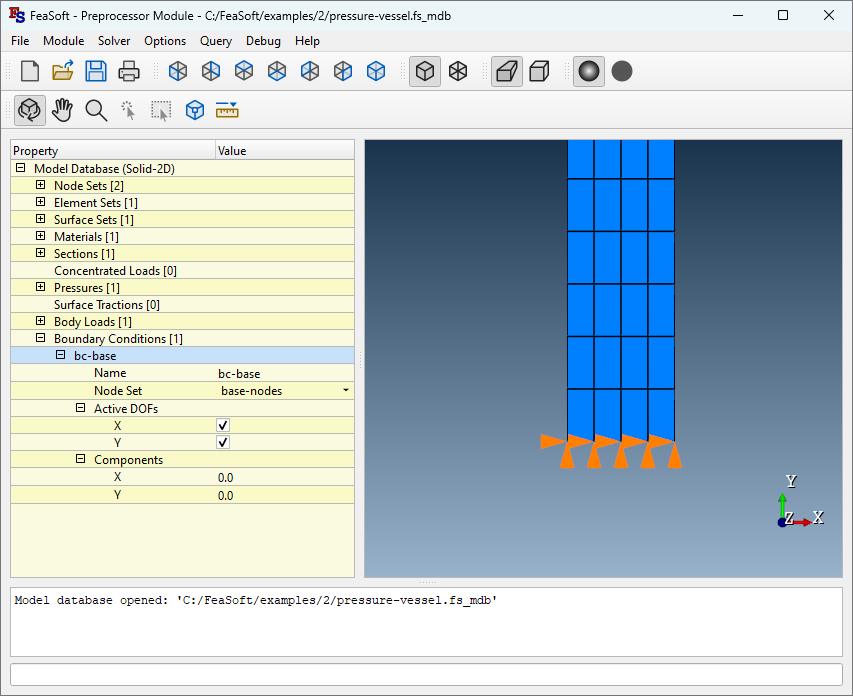
\includegraphics[scale=0.5]{fig/ui-2-11.png}
\end{center}

\textbf{Important:} since the model has been completely defined, it is necessary to save it now (File > Save or via the Save Model Database toolbar button) before submitting the job to the solver; the preprocessor will always consider the last saved state of the model (unsaved changes are ignored for the analysis).

Following the same procedure used in the first example, submit the model to a static analysis and, once completed, plot the Mises Equivalent Stress nodal scalar field:
\begin{center}
    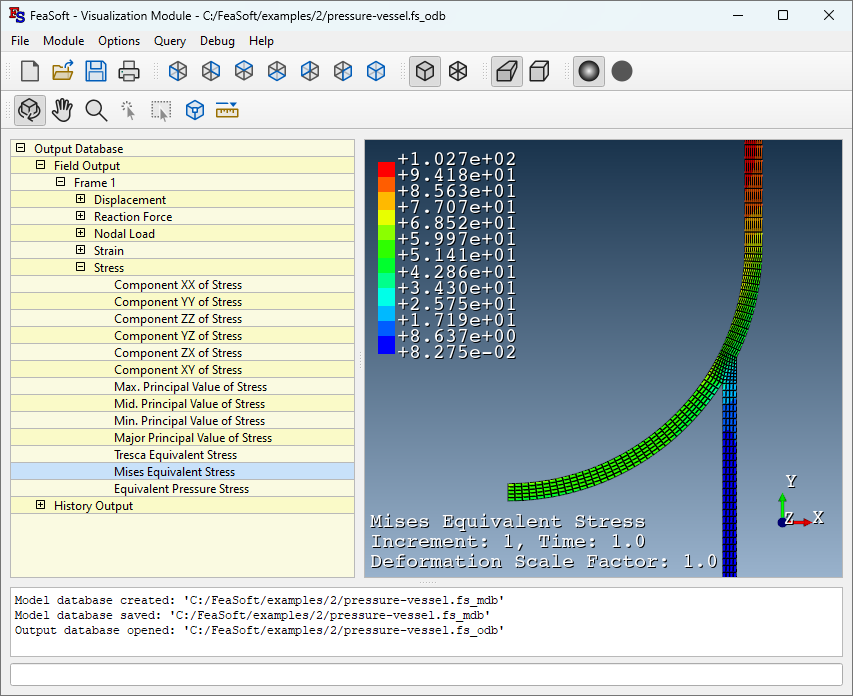
\includegraphics[scale=0.5]{fig/ui-2-12.png}
\end{center}

As previously mentioned, several options can be adjusted on the Options > Common and Options > Result dialogs. The viewport can also be printed via the File > Print...\ menu action or the Print Viewport toolbar button. An example on how the results can be presented is shown below:
\begin{center}
    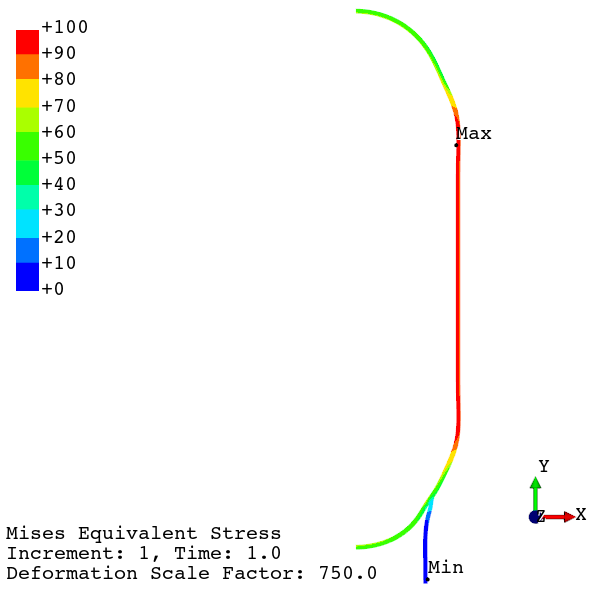
\includegraphics[scale=0.5]{fig/ui-2-13.png}
\end{center}

\subsection{Frequency analysis of a fixed plate}

Consider a rectangular plate with a length of $a = 200$ mm, a width of $b = 180$ mm, and a thickness of $t = 10$ mm. The plate's material is considered linear-elastic, defined by a Young's modulus of $E = 210$ GPa, a Poisson's ratio of $\nu = 0.3$, and a mass density of $\rho = 7.85$ g/cm\textsuperscript{3}. The plate is fixed on all its sides. The objective is to obtain the normal modes of vibration assuming a general three-dimensional case.

\textbf{Important:} before starting the model definition, always remember that FeaSoft, like other finite element applications (e.g., Abaqus), assumes that consistent units are used. For this example, the geometric properties are specified in mm, while the Young's modulus is specified in MPa, i.e., N/mm\textsuperscript{2}; moreover, the density is specified in t/mm\textsuperscript{3}. Consequently, displacements\footnote{Mode shapes are normalized with respect to the mass matrix of the system (as customary).} will be computed in mm and frequencies will be computed in Hz (or cycles/s).

To start the model definition in FeaSoft, go to File > New...\ and open the pre-prepared mesh input file named fixed-plate.inp found in the examples/3 directory. The application should warn that a model database already exists in the directory; press Yes on the dialog box to proceed. The newly created model database should be displayed in the interface as shown:
\begin{center}
    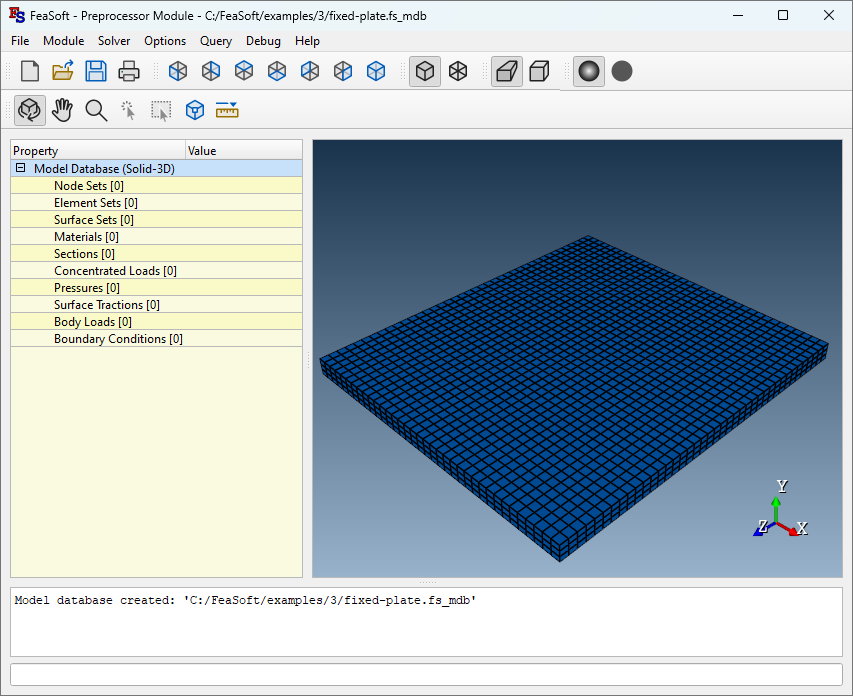
\includegraphics[scale=0.5]{fig/ui-3-1.png}
\end{center}

In the toolbar, click the View Top button, the Cell Wireframe Representation button, and the Parallel Projection button:
\begin{center}
    \begin{tikzpicture}
        \node[inner sep=0] at (0,0) {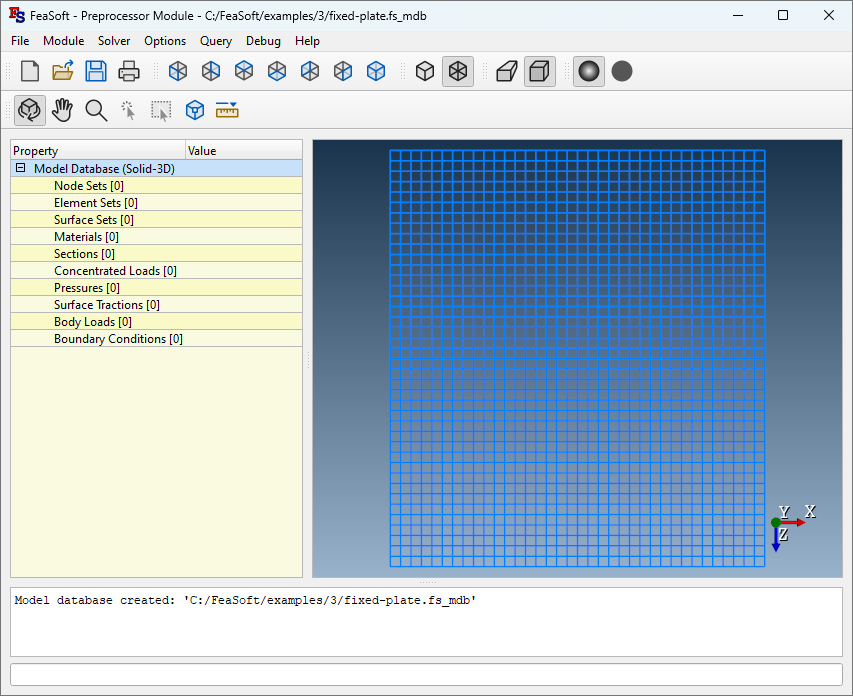
\includegraphics[scale=0.5]{fig/ui-3-2.png}};
        \draw[red] (-2.65,3.4) rectangle (-2.17,3.92);
        \draw[red] (0.16,3.4) rectangle (0.655,3.92);
        \draw[red] (1.25,3.4) rectangle (1.745,3.92);
    \end{tikzpicture}
\end{center}
It is often convenient to enable parallel projection when picking on 3D views in order to avoid picking unwanted nodes or elements, which may happen due to perspective effects if perspective projection is active. Additionally, enabling a wireframe cell representation allows the user to visualize if internal nodes or elements are picked.

Using the techniques learned so far, create the following node set named Side-Nodes, which should contain exactly 608 nodes:
\begin{center}
    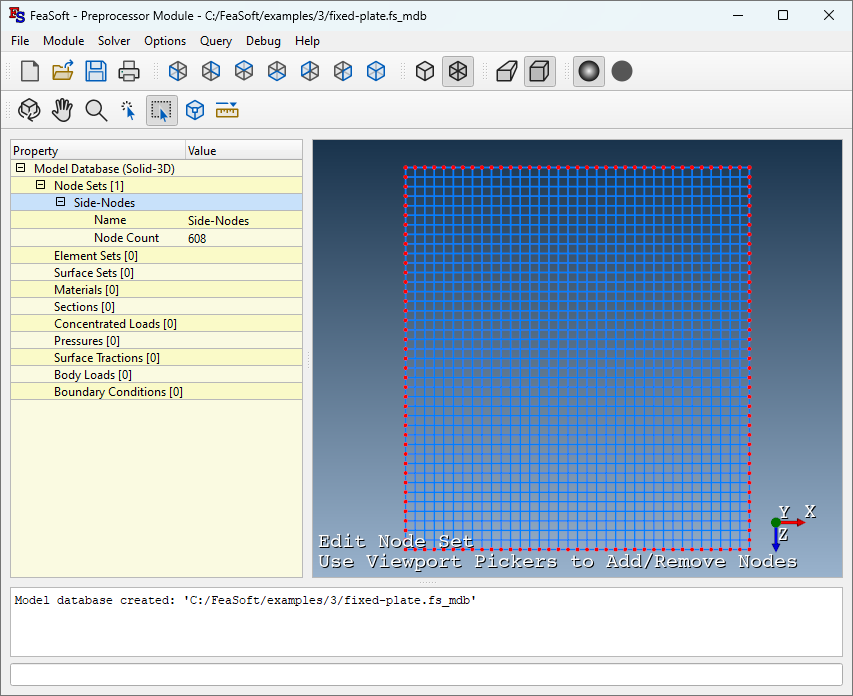
\includegraphics[scale=0.5]{fig/ui-3-3.png}
\end{center}

Select the Cell Surface Representation and Perspective Projection toolbar buttons, and use the Rotate interaction style to verify that the side nodes are selected:
\begin{center}
    \begin{tikzpicture}
        \node[inner sep=0] at (0,0) {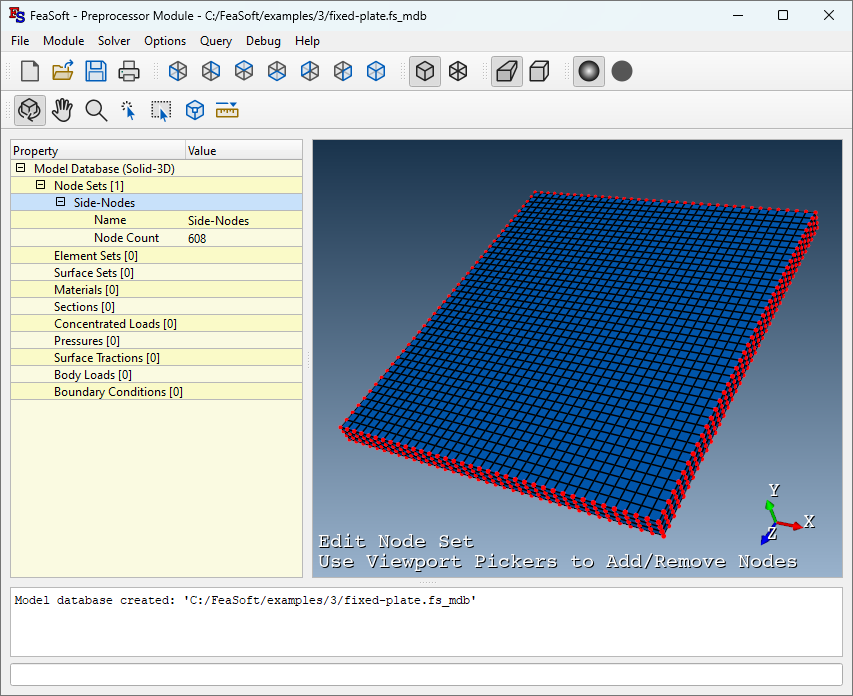
\includegraphics[scale=0.5]{fig/ui-3-4.png}};
        \draw[red] (-5.5,2.9) rectangle (-5.0,3.4);
        \draw[red] (-0.25,3.4) rectangle (0.195,3.92);
        \draw[red] (0.85,3.4) rectangle (1.275,3.92);
    \end{tikzpicture}
\end{center}

Create an element set named All-Elements, which includes all 4320 elements:
\begin{center}
    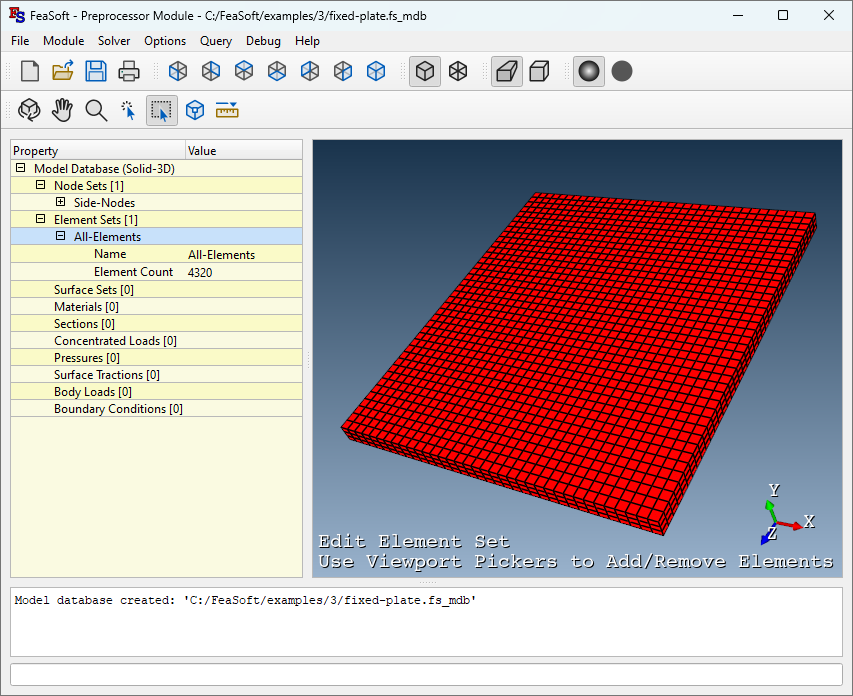
\includegraphics[scale=0.5]{fig/ui-3-5.png}
\end{center}

Create the following material and section:
\begin{center}
    \begin{tikzpicture}
        \node[draw=red,inner sep=0.5] at (0,0) {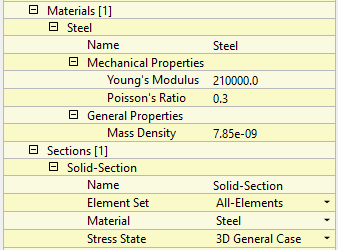
\includegraphics[scale=1]{fig/ui-3-6.png}};
    \end{tikzpicture}
\end{center}

Create the following boundary condition:
\begin{center}
    \begin{tikzpicture}
        \node[draw=red,inner sep=0.5] at (0,0) {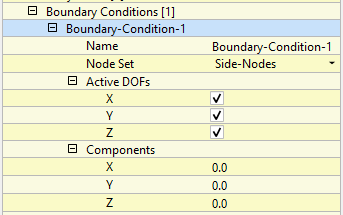
\includegraphics[scale=1]{fig/ui-3-7.png}};
    \end{tikzpicture}
\end{center}
\begin{center}
    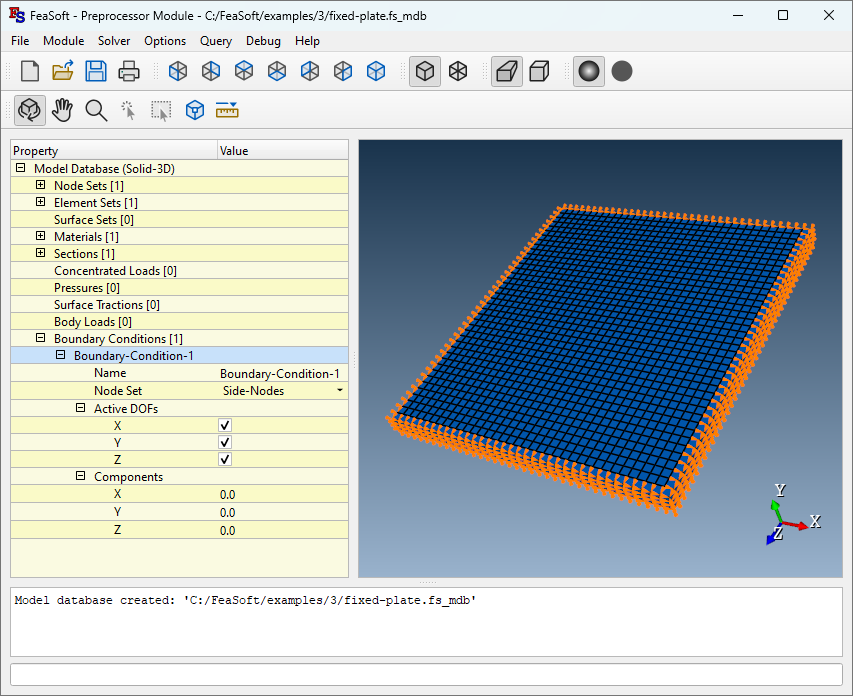
\includegraphics[scale=0.5]{fig/ui-3-8.png}
\end{center}

\textbf{Important:} since the model has been completely defined, it is necessary to save it now (File > Save or via the Save Model Database toolbar button) before submitting the job to the solver; the preprocessor will always consider the last saved state of the model (unsaved changes are ignored for the analysis).

Submit a frequency analysis, requesting the first 10 eigenpairs, i.e., the first 10 normal modes of vibration:
\begin{center}
    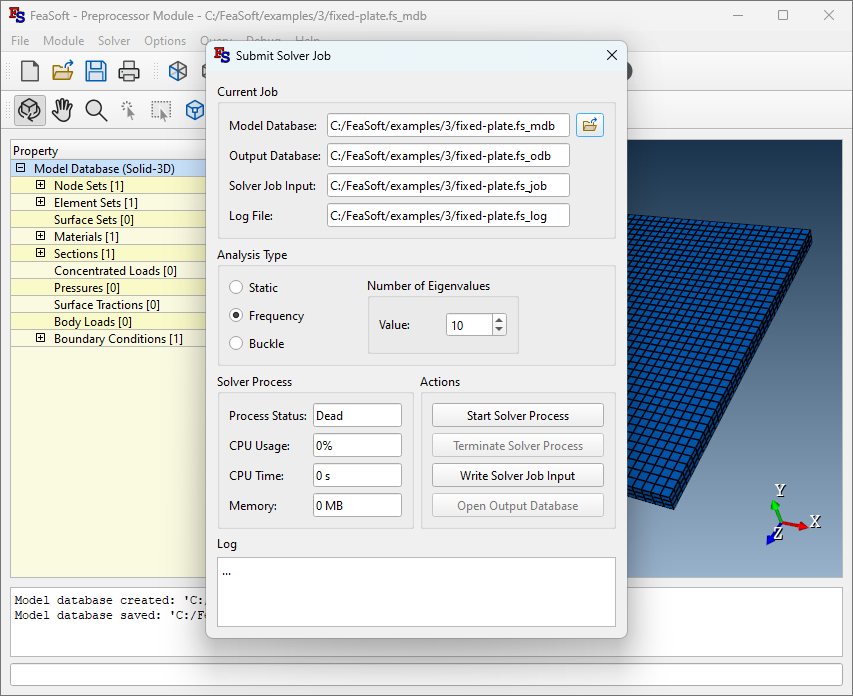
\includegraphics[scale=0.5]{fig/ui-3-9.png}
\end{center}

Once the analysis has been completed, plot, for example, the 4th mode shape:
\begin{center}
    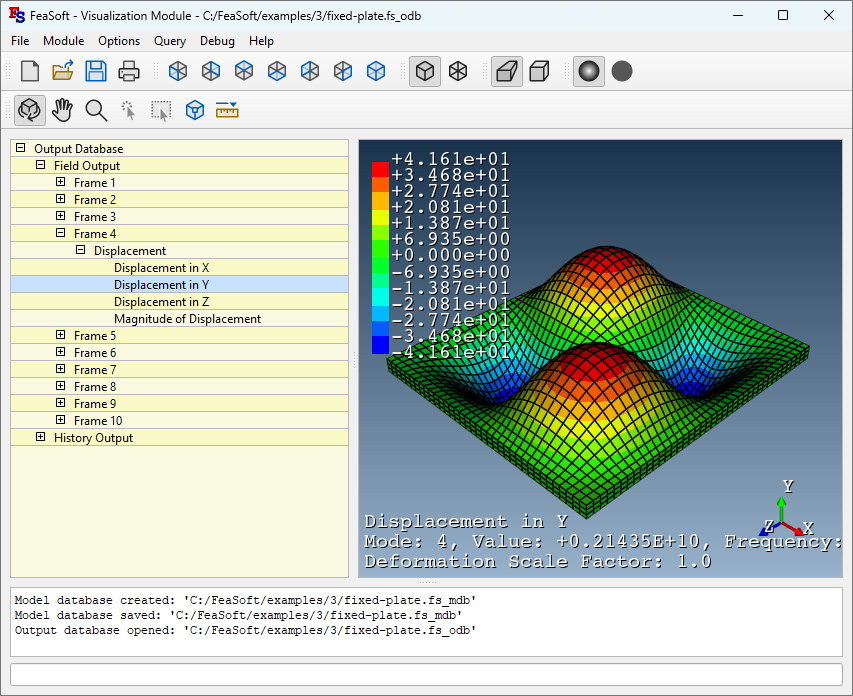
\includegraphics[scale=0.5]{fig/ui-3-10.png}
\end{center}

As previously mentioned, several options can be adjusted on the Options > Common and Options > Result dialogs. The viewport can also be printed via the File > Print...\ menu action or the Print Viewport toolbar button. An example on how the results can be presented is shown below:
\begin{center}
    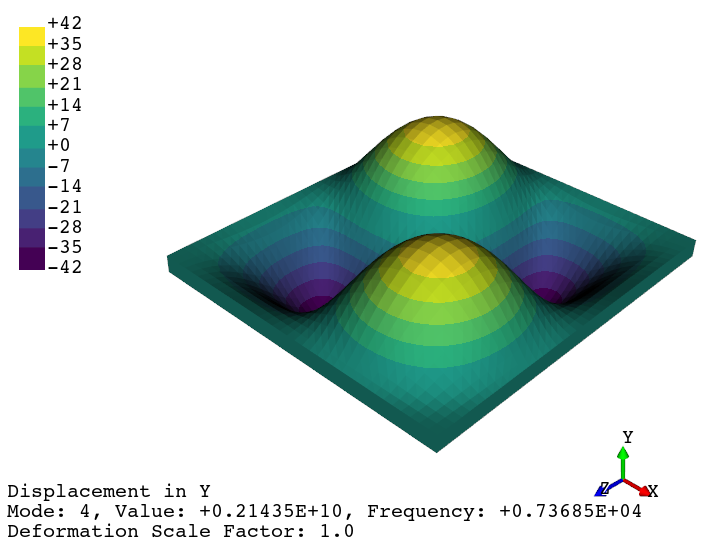
\includegraphics[scale=0.5]{fig/ui-3-11.png}
\end{center}

\subsection{Buckle analysis of a column}

Consider the following problem:
\begin{center}
    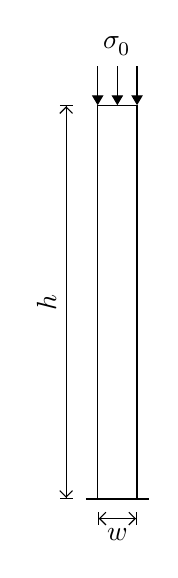
\begin{tikzpicture}[scale=1]
        \draw (-0.25,0) rectangle (0.25,5);
        \draw[thick] (-0.4,0) -- (0.4,0);
        \draw[Triangle-] (-0.25,5) -- ++(90:0.5);
        \draw[Triangle-] (+0.00,5) -- ++(90:0.5) node[above]{$\sigma_0$};
        \draw[Triangle-] (+0.25,5) -- ++(90:0.5);
        \draw[{Bar}{Straight Barb}-{Straight Barb}{Bar}] (-0.65,0) -- (-0.65,5) node[midway,rotate=90,above]{$h$};
        \draw[{Bar}{Straight Barb}-{Straight Barb}{Bar}] (-0.25,-0.25) -- (0.25,-0.25) node[midway,below]{$w$};
    \end{tikzpicture}
\end{center}
The geometry of the column is defined by a span of $l = 50$ m, a height of $h = 5$ m, and a width of $w = 1$ m. The material is considered linear-elastic, defined by a Young's modulus of $E = 210$ GPa and a Poisson's ratio of $\nu = 0.3$. The compression load has a magnitude of $\sigma_0 = 1$ MPa, as the objective is to compute the load multiplier (an eigenvalue) for which the column is expected to buckle under the considered load pattern. A plane strain condition is assumed.

\textbf{Important:} before starting the model definition, always remember that FeaSoft, like other finite element applications (e.g., Abaqus), assumes that consistent units are used. For this example, the geometric properties are specified in mm, while the Young's modulus and the compression load are specified in MPa, i.e., N/mm\textsuperscript{2}. Consequently, displacements\footnote{Buckle shapes are normalized with respect to the norm of the eigenvector.} will be computed in mm.

To start the model definition in FeaSoft, go to File > New...\ and open the pre-prepared mesh input file named column.inp found in the examples/4 directory. The application should warn that a model database already exists in the directory; press Yes on the dialog box to proceed. The newly created model database should be displayed in the interface as shown:
\begin{center}
    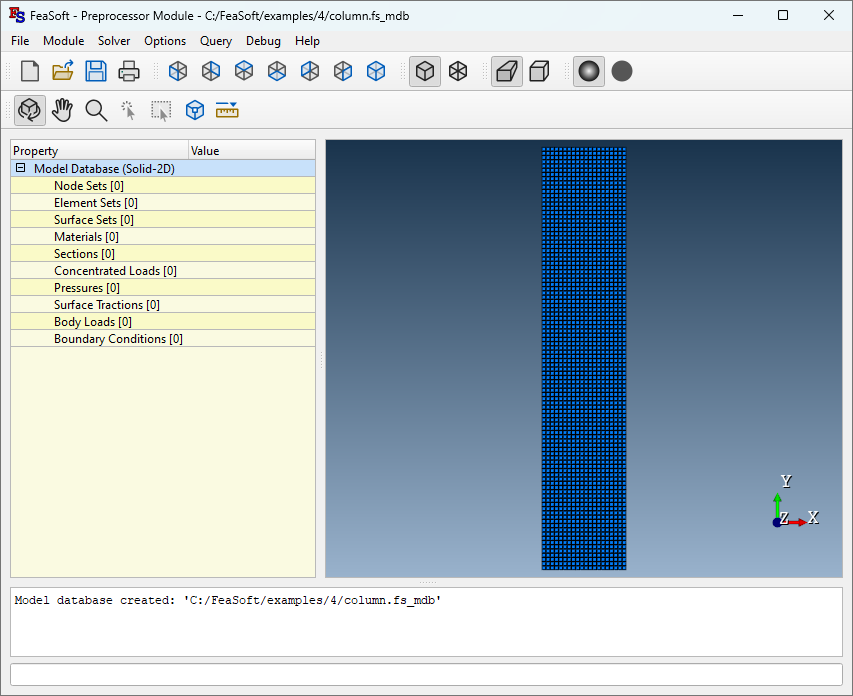
\includegraphics[scale=0.5]{fig/ui-4-1.png}
\end{center}

Using the techniques learned so far, create the following node set named Bottom-Nodes, which should contain exactly 21 nodes:
\begin{center}
    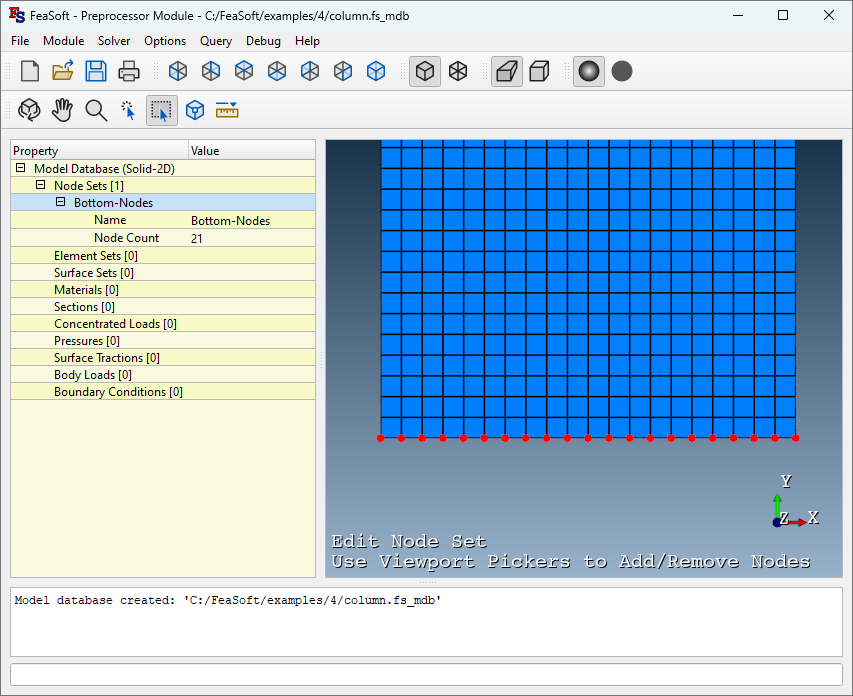
\includegraphics[scale=0.5]{fig/ui-4-2.png}
\end{center}

Create the following element set named All-Elements, which should contain all 2000 elements:
\begin{center}
    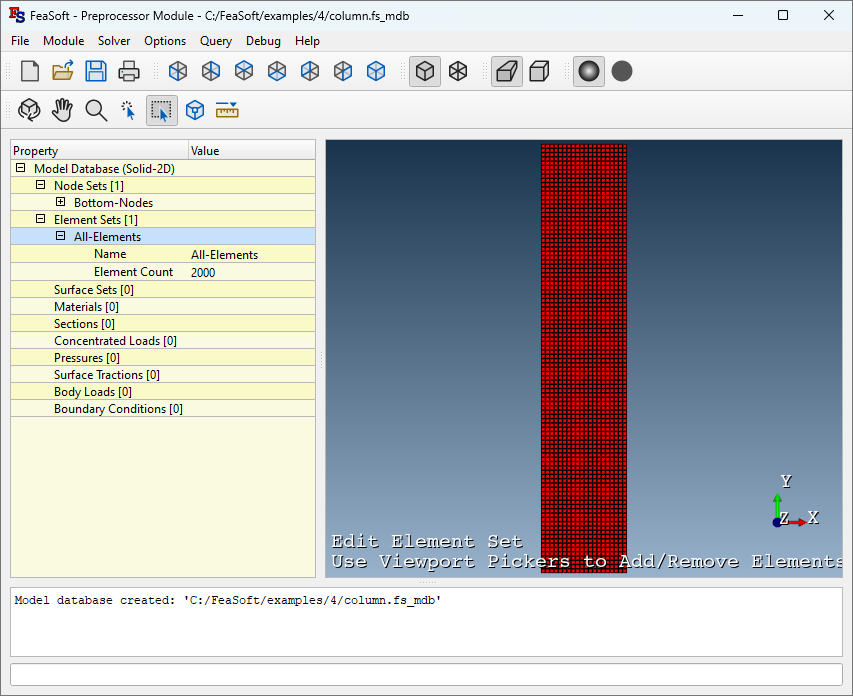
\includegraphics[scale=0.5]{fig/ui-4-3.png}
\end{center}

Create the following surface set named Load-Surface, which should contain exactly 20 element surfaces:
\begin{center}
    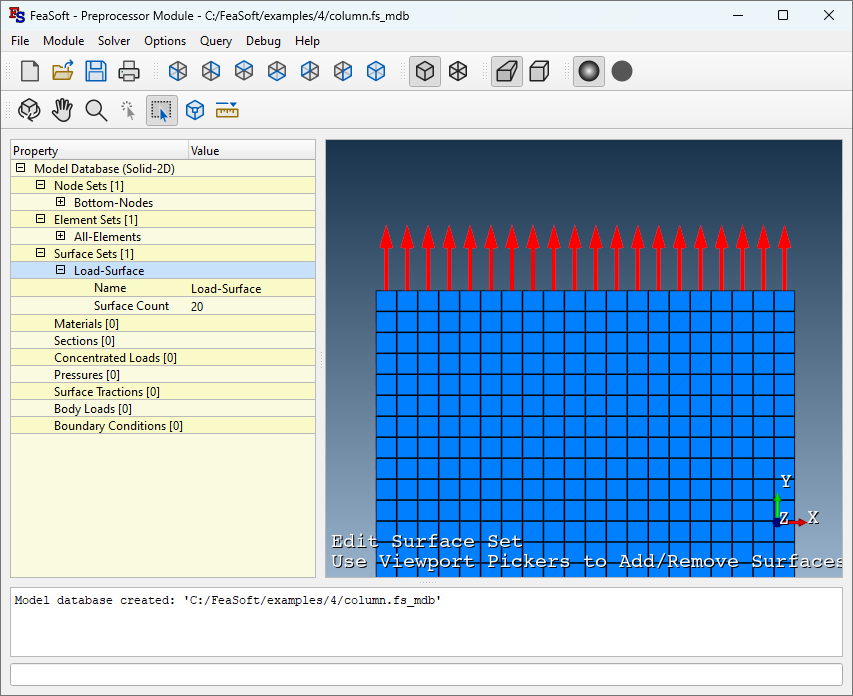
\includegraphics[scale=0.5]{fig/ui-4-4.png}
\end{center}

Create the following material and section:
\begin{center}
    \begin{tikzpicture}
        \node[draw=red,inner sep=0.5] at (0,0) {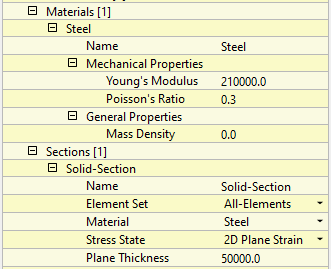
\includegraphics[scale=1]{fig/ui-4-5.png}};
    \end{tikzpicture}
\end{center}

Create the following pressure:
\begin{center}
    \begin{tikzpicture}
        \node[draw=red,inner sep=0.5] at (0,0) {\includegraphics[scale=1]{fig/ui-4-6.png}};
    \end{tikzpicture}
\end{center}
\begin{center}
    \includegraphics[scale=0.5]{fig/ui-4-7.png}
\end{center}

Create the following boundary condition:
\begin{center}
    \begin{tikzpicture}
        \node[draw=red,inner sep=0.5] at (0,0) {\includegraphics[scale=1]{fig/ui-4-8.png}};
    \end{tikzpicture}
\end{center}
\begin{center}
    \includegraphics[scale=0.5]{fig/ui-4-9.png}
\end{center}

\textbf{Important:} since the model has been completely defined, it is necessary to save it now (File > Save or via the Save Model Database toolbar button) before submitting the job to the solver; the preprocessor will always consider the last saved state of the model (unsaved changes are ignored for the analysis).

Submit a buckle analysis, requesting the first 5 eigenpairs, i.e., the first 5 buckling modes:
\begin{center}
    \includegraphics[scale=0.5]{fig/ui-4-10.png}
\end{center}

Once the analysis has been completed, plot, for example, the 2nd buckle shape:
\begin{center}
    \includegraphics[scale=0.5]{fig/ui-4-11.png}
\end{center}

As previously mentioned, several options can be adjusted on the Options > Common and Options > Result dialogs. The viewport can also be printed via the File > Print...\ menu action or the Print Viewport toolbar button. An example on how the results can be presented is shown below:
\begin{center}
    \includegraphics[scale=0.5]{fig/ui-4-12.png}
\end{center}

\end{document}
